% Chapter 3
%
\chapter{Concept and Design of SendIt} % Main chapter title
%
	%Concepts
		%First trust
		%Trust building & factors (timing etc)
		%Authentication
			


\label{Chapter3} % For referencing the chapter elsewhere, use \ref{Chapter1} 
%
This chapter will discuss the overall concepts and design of SendIt. It will illustrate how SendIt utilizes the solutions discussed in \Cref{Chapter2} and how this is beneficial to the system as a whole. In addition, general information relevant to the application and system will be discussed here. It will also discuss the design of the ACS server.

%
\section{Concepts}
%Concepts
%
The following concepts and assumptions build the base of how the technology is applied, while also being a product of the technological limitations and how this technology is implemented. The concepts introduced are a mix of new concepts and ideas and concepts borrowed from previous research. The assumptions are a result, and consequence, of the initial idea of the system, as well as the technological limitations imposed by the chosen technologies, combined with the lack of better options. These assumptions were necessary to narrow down the work and to be able to keep the system simple for the end users. While these assumptions may limit or reduce some of the security measures available, the limitations they would impose on the usability were considered more important.

%
	\subsection{First trust}
		%
		The first trust, or initial trust, is the basis of every interaction in every computer system, as well as in the real world. In the real world, you can see the other person, and as such, easily identify who it is. This is not the case in computer systems, therefore, a way to identify entities is necessary. In this system, the choice was made to use e-mail addresses as a basis for uniquely identifying each entity. Since one of the main goals is to improve e-mail attachments, it felt like a natural choice, as well as being easy to implement. Since there is now a way to address each entity, the necessity for confirming that identity arises. This process is called authentication, and how it is done will be discussed more in-depth later.

		To be able to authenticate an identity, the fact that the identity has to possess something unique has to be addressed. If not, someone else can impersonate them. In the real world, everyone has a unique (or close to unique) appearance, which is almost impossible to fake. This is not the case for computers. Usually the PKI model (explained in \Cref{sec:pkc}), is used to vouch for the validity of an identity in computer systems. As explained previously, this requires a lot of setup and cannot be done easily. Because of this, it is not fit to be used in combination with SendIt. 

		SendIt is built on the idea of trusting the first interaction, based on non-absolute authentication methods. This means the first Answer and Offer exchange (connection setup) is done assuming the other endpoint is not malicious. It is done in an unencrypted manner, without any guarantee of the integrity of the message or using any authentication mechanisms. The reason for choosing this solution is that it allows for an easy and convenient way to start communicating with new partners. It is important that the system is kept simple, to keep it user friendly.

		It also allows for an intuitive approach to the first interaction. Instead of having someone's pre-shared secret or other means of authentication, the timing and files shared can be a means of authentication. It feels unnatural to have someone randomly send files to you, unless it is somewhat expected. It is also strange to receive files where the content seems unknown or strange, without any previous communication or knowledge. As such, the argument can be made that this system is more intuitive than the alternatives.

		While the timing and files shared do continue to count towards the trustworthiness of an identity, it is important to note that \emph{only the first interaction is inherently trusted}. All subsequent communication is end-to-end encrypted and the endpoint is \emph{always authenticated} before communication starts. As such, if the user takes care to be certain of the endpoints identity for the first interaction, all subsequent interactions are guaranteed to be with the same identity, barring that user having their credentials stolen.

		The take away from this is, while the timing and files shared should still be considered, all subsequent interactions are, by and large, guaranteed to be with the same identity. As such users are encouraged to take extra care during the initial setup, but can relax and trust the endpoint during all future interactions and rely on the system to warn them if something is amiss.

		To sum it up by using a comparative example: If someone were to place a random package outside your door at a random time, with no information on it, one would naturally be wary of the contents and motives of that person. In contrast, if a friend made an appointment to deliver a package that day, one would be much less suspicions, even if it was identical to the package described in the previous scenario. There is no guarantee that the package is from your friend, but it is likely.

		This is the basis of the first trust in SendIt, and allows for an unauthenticated interaction to be the basis of the trust building.  The added benefit is that unlike in the real world, SendIt can guarantee that the package is unaltered and from your friend for \emph{every interaction after the first one}, no matter when it is delivered and what the package may look like.

		There is no denying that this decision leaves the system and end user open to be attacked during this first interaction. The advantage is that it keeps the system easy to use, and allows for a relatively secure system, which relies on human and intuitive factors for establishing the first trust. It relies on machine made, absolute authentication from that point on.

	%
	\subsection{Trust building}
		%
		Trust building in the suggested system, is based on several factors. Before getting into the specifics, it is necessary to point out that the trust system is only a theoretical approach and has not been implemented in the prototype. The proposed system uses trust transitivity \cite{lcns_semantic} (\emph{Trusting in Alice and Alice trusting Bob, means that we trust Bob more, than if Alice was not involved}).

		Other means of building trust includes frequency of communication and bi-directional communication (Acting as both sender and receiver with the same identities involved). Trust built by such activities will gradually accumulate, in contrast to transitive trust. Transitive trust is just a way of assigning an identity a trust level based on the introducers of that identity, and their respective level of trust in said identity. (\emph{How many trusted identities signed, how much do we trust those identities and how much do they trust the certificate?})

		Trust can also be reduced. One event that can cause this is if a user tries to communicate with a previous partner, but that partner is not authenticated according to the key associated with that partner. SendIt's trust system works in a way that gives more weight to reduction in trust. This means it will be harder to gain trust, than to lose it. This is because it is generally a safer approach to be wary, than to assume good faith. In other words, a negative incident will reduce the trust significantly more than a positive incident will increase it. This will help maintain a balanced system that detects untrusted behavior rapidly and acts accordingly.

		%\paragraph{}
		Trust is shared by using certificates. Unlike regular certificates (see \Cref{sec:cert}), SendIt proposes a minimal and simple solution. It proposes that a certificate is just a list of identities and the corresponding cipher. The cipher is made by encrypting the public key of the identity being vouched for, with the users own private key. This way all that is needed to verify the authenticity of a key, is to find the introducer's public key and decrypt the cipher. As such, certificates will contain these fields: Introducer's name, Cipher, and Trust. The cipher is as just described. The trust field is a value of either 1 or 2, where 1 indicates full trust and 2 indicates partial trust. The trust value is included so it is possible to assess how much trust the introducer has in the introduced key.
		%
		\begin{figure}
		  \centering
		  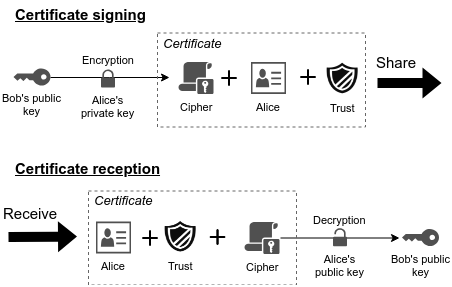
\includegraphics[width=85mm]{Certificate_explained}\\
		  \vspace{1cm}
		  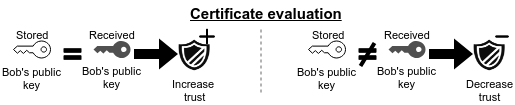
\includegraphics[width=85mm]{Certificate_eval}
		  \centering
		  \decoRule
		  \caption[Certificate transfer and evaluation]{Certificate operations example where Alice signs Bob's certificate.}
		  \label{fig:cert_ex}
		\end{figure}
		%

		When it comes to transitive trust, the specific values and model for assigning trust is not specified, but the idea is to assign different levels of trust, based on the amount of introducers from different trust levels. The level of trust a user has in the introducer of a certificate, directly affects the trust level given to the certificate.

		Once an endpoint has received the certificates, they will be evaluated based on the signatures attached and potentially existing trust values. When the value has been calculated and the new trust level assigned, the key is available like any other and will be used in communications with that identity. See \Cref{fig:cert_ex} for an example. Do note that one certificate can hold many signatures.

		%\paragraph{}
		The practical evaluation scheme for the system is not implemented in SendIt, but the initial idea was to assign these trust-levels based on a point system, where an identity accumulates points by getting verified by introducers that the user trusts. An option is to have different levels of trust, where an identity is assigned a trust level according to the amount of points it has accumulated.

		The amount of points granted for each introducer depends on the trust level the user assigns to the introducer. It also depends on how much this introducer trusts in the key. This is so the nuance of transitive trust is clearer, since the system is based on these nuances of trust. SendIt should have an easy and intuitive trust evaluation, while also having a simple way to fairly assert the trust level of an identity. Unlike the web of trust model, different levels of trust for communication and for introducing keys should not be applied. There should only be one trust level assigned to each identity and it should apply to both uses equally.

		The practical impact of the different trust levels should be visible to the user as a warning, if the receiver does not have a trust level that is sufficient according to the users settings. The user should be able to choose if he wants to ignore the warning or cancel the transfer. If the receiver meets the requirements, no notifications or warnings should appear.

		SendIt should come with pre-configured values so novice users can rely on the standard settings. If they want to change these settings, they should have the option to choose to do so. The users should have an overview of all identities and should also have an overview of the respective trust-levels available in the settings menu, and the option to manually change these levels. This allows the users to override the system in cases where they deem themselves better equipped to evaluate the trust-level of the identity.

		%\paragraph{}
		As noted in \Cref{sec:trust_syb}, the Sybil attack is a problem in decentralized, reputation based networks. The proposed system will not be completely immune to such attacks, but instead look towards making it hard to propagate and become regarded as trustworthy by the majority of identities. This will be achieved by requiring interactions with other identities, as well as a signed certificate from trusted introducers, to gain a high level of trust. By requiring these, in combination, an attacker can not simply create a large sub-network of controlled identities that all trust each other, and then spread it to the main network with the same level of trust.

		This allows for high resistance against this attack, since the attack exploits the fact that a large number of untrusted identities can manipulate how the main network regards the attacker. Since none of these identities will have a high amount of trust in the main network, they will not be regarded as safe. This is true even if they have a large amount of introducers, because the introducers are untrusted identities as well.

	%
	\subsection{Authentication}
		%Authentication

		The authentication scheme in SendIt is based on public-key cryptography. Each identity, or e-mail address if you will, is associated with a unique public and private key. These key pairs are used for authentication. In practice, this is done by encrypting the Offer and the Answer used to establish the WebRTC connection with the other endpoint's public key. This way the ability to connect to each other also acts as authentication, since only the identity with the correct private key can access the information. This explanation is a slight simplification and will be discussed in detail in \Cref{sec:crypto_des}.

		This is in contrast to usual solutions, where authentication is done before initiating a connection. SendIt's solution removes the extra step, and combines these two processes into one. The reason this is made possible is because of how WebRTC's connection setup is done. Because of the authentication built into the Offer and Answer exchange, the system guarantees authentication of both endpoints. For more details on WebRTC's built in authentication of endpoints, see \Cref{sec:conn_setup}.

		As recently noted, the authentication in SendIt relies on key pairs. The key associated with an identity is shared during the first interaction. While there is no authentication of the respective identities during this interaction, the keys are shared over the P2P channel. This channel is end-to-end encrypted, as to not be vulnerable to attacks that manipulate the data in transit. In summary, as long as you connect to the correct endpoint in your first interaction, there is no reasonable way an attacker can impersonate that endpoint at a later time.

		It is also important to note that while the proposed system suggests using e-mail addresses as identifiers, there is no direct connection between the identities in the system and the actual e-mail system. By using e-mail addresses, it makes it easier to add extra trust, by implementing an e-mail verification step if desired. The consequence of this initial separation does mean that the e-mail system has no direct influence or inherent effect on SendIt, but their close relation makes it easy to link the two. This gives all the benefit of the e-mail system, while not having to consider the risks or threats that are inherent to that system. It is left up to the developers and users of SendIt to decide if they believe such a link is a positive or negative addition, and as such their choice to make.
%
%Des
\section{System design}
%SendIt implementation
%
The following section will address the design of the general solutions used in SendIt. It will explore the functionality that is used for both modes, and explain how they work and why they are necessary. It will also build the basis for understanding how the two modes operate, and which functions they build upon in order to work.

	%
	\subsection{Cryptography}
	\label{sec:crypto_des}
%
	\begin{figure}[th]
	  \centering
	  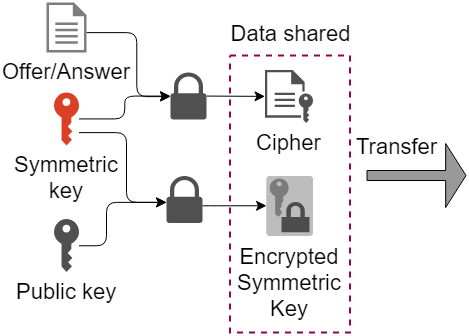
\includegraphics[width=100mm]{Figures/Encrypt}
	  \decoRule
	  \caption[Authentication exchange: Encryption]{In this figure it is shown how the Offer/Answer is encrypted with a symmetric key, creating a cipher. This symmetric key is then encrypted with the recipients public key. The cipher and the encrypted key are then shared.}
	  \label{fig:enc}
	\end{figure}
	\begin{figure}[th]
	  \centering
	  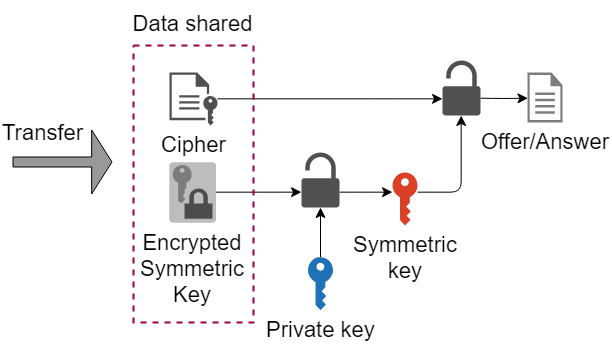
\includegraphics[width=100mm]{Figures/Decrypt}
	  \decoRule
	  \caption[Authentication exchange: Decryption]{Here one can see the received data and how it is decrypted back into the original Offer/Answer. Only the identity with the correct private key can access the original data.}
	  \label{fig:decr}
	\end{figure}

	When a new key pair is created it is not stored on the disk until the public key has been successfully exchanged with another identity, in order to avoid storing unnecessary keys. The file where the keys are stored should be password protected, or otherwise encrypted, to ensure that if it is stolen, it takes considerable effort to steal the keys.

	SendIt also utilizes symmetric keys for encrypting data. These symmetric keys are generated for every session, and used for one session only. The reason symmetric keys are necessary, is because the amount of data that can be encrypted with public-key cryptography is fairly small, and as such, a solution which can encrypt more data is needed.

	The biggest difference between the symmetric keys and the asymmetric key pairs in SendIt, is that the symmetric keys are not stored across multiple sessions. The asymmetric keys however, are stored and stay the same. This is because they are used for authenticating the identities. The way this is done is in a similar fashion to standard PGP encryption and decryption, as explained in \Cref{sec:pgp_enc}. See \Cref{fig:enc} and \Cref{fig:decr} for illustrations on, respectively, encryption and decryption.

	The plaintext in this case is the Offer or the Answer. If it is encrypted, it also contains the encrypted symmetric key, as well as the initialization vector for that key. The initialization vector consists of random integers. The IV is needed to correctly decrypt the data. 

	The difference between SendIt and PGP is that in order to authenticate the Sender, the Recipient needs to encrypt the IV with the Sender's public key and transfer this. If a connection is made, it means both endpoints had to have the correct keys. This is because of the way the connection setup works, as described in \Cref{sec:webrtc_off}.

	\subsection{Protocol}
	%FT protocol
		%How? Which fields? Additions?
	The base protocol used in SendIt is based on the one used in PubShare, an online WebRTC P2P file transfer solution \cite{url_pubshare}. This protocol has been extended and altered to fit with SendIt's needs. This protocol takes care of communicating the status of the file transfer, chunking the data, sharing file metadata, and verification of transfer completion. The protocol is also in charge of setting up authentication of the endpoints, since the data to authenticate eachother should be exchanged directly. This protocol is very limited, and as such, unlikely to have a large overhead and impact on performance, however, this is only an assumption. Following will be a description of the different functionalities of the protocol.

	\subsubsection*{Authentication setup}
	The authentication setup functionality consists of an Authentication setup packet and an Authentication setup reply packet. Both of these packets contain the identity and their associated public key. If one of these packets are received, the system checks that the information supplied does not conflict with existing data. If it does not, and the packet was of the type Authentication setup, the endpoint creates an Authentication setup reply packet and sends it back. If it was of the type Authentication setup reply, the transfer is initiated.

	\subsubsection*{Offer and Answer}
	The Offer packet contains metadata about the files to be sent, so the recipient knows how many files will be transferred, what type of files they are, and how big they are. The Answer packet is just a confirmation that this data was received and that the recipient is getting ready for the transfer.

	\subsubsection*{Request and Data}
	Once the recipient is ready to receive the first data, a Request packet is sent indicating which chunks it wants to receive. It is also used to confirm which packets it has previously received, and to request more data once all the previous chunks have been received. The Data packet contains information about which chunk is being sent, and the file-data for that chunk - the part of the file currently being transferred.

	Following is an example to illustrate how it works: The recipient sends a Request packet requesting chunks 10 through 20. This also confirms all chunks up until 10 is complete. The Sender then transfers these chunks to the Recipient. Once all chunks are received, it requests more chunks until all chunks have been received. If a chunk is not received, the chunk before is treated as the last chunk received, and the chunks afterwards are re-transmitted.

	\subsubsection*{Done}
	The Done packet contains no data field, and is a confirmation that the Recipient has received the file currently being transferred. If there are no more files to transfer, this indicates the end of the connection. If more files are waiting, transfer of the next file will begin once this packet is received.

	\subsubsection*{Cancel and Error}
	The Cancel packet is sent if the user for some reason decides to cancel the current transfer. This interrupts the transfer and closes the connection. If the Error packet is sent, it means an error occurred and the transfer is stopped and the connection closed.

	\subsubsection*{Request metadata}
	The Request metadata packet is only used in the ACS mode. It is necessary so the Recipient can request data about which files are being offered by the Sender, before accepting the connection. 

	%
	\subsection{File transfer functionality}
	%File transfer
		%
		\begin{figure}[th]
		  \centering
		  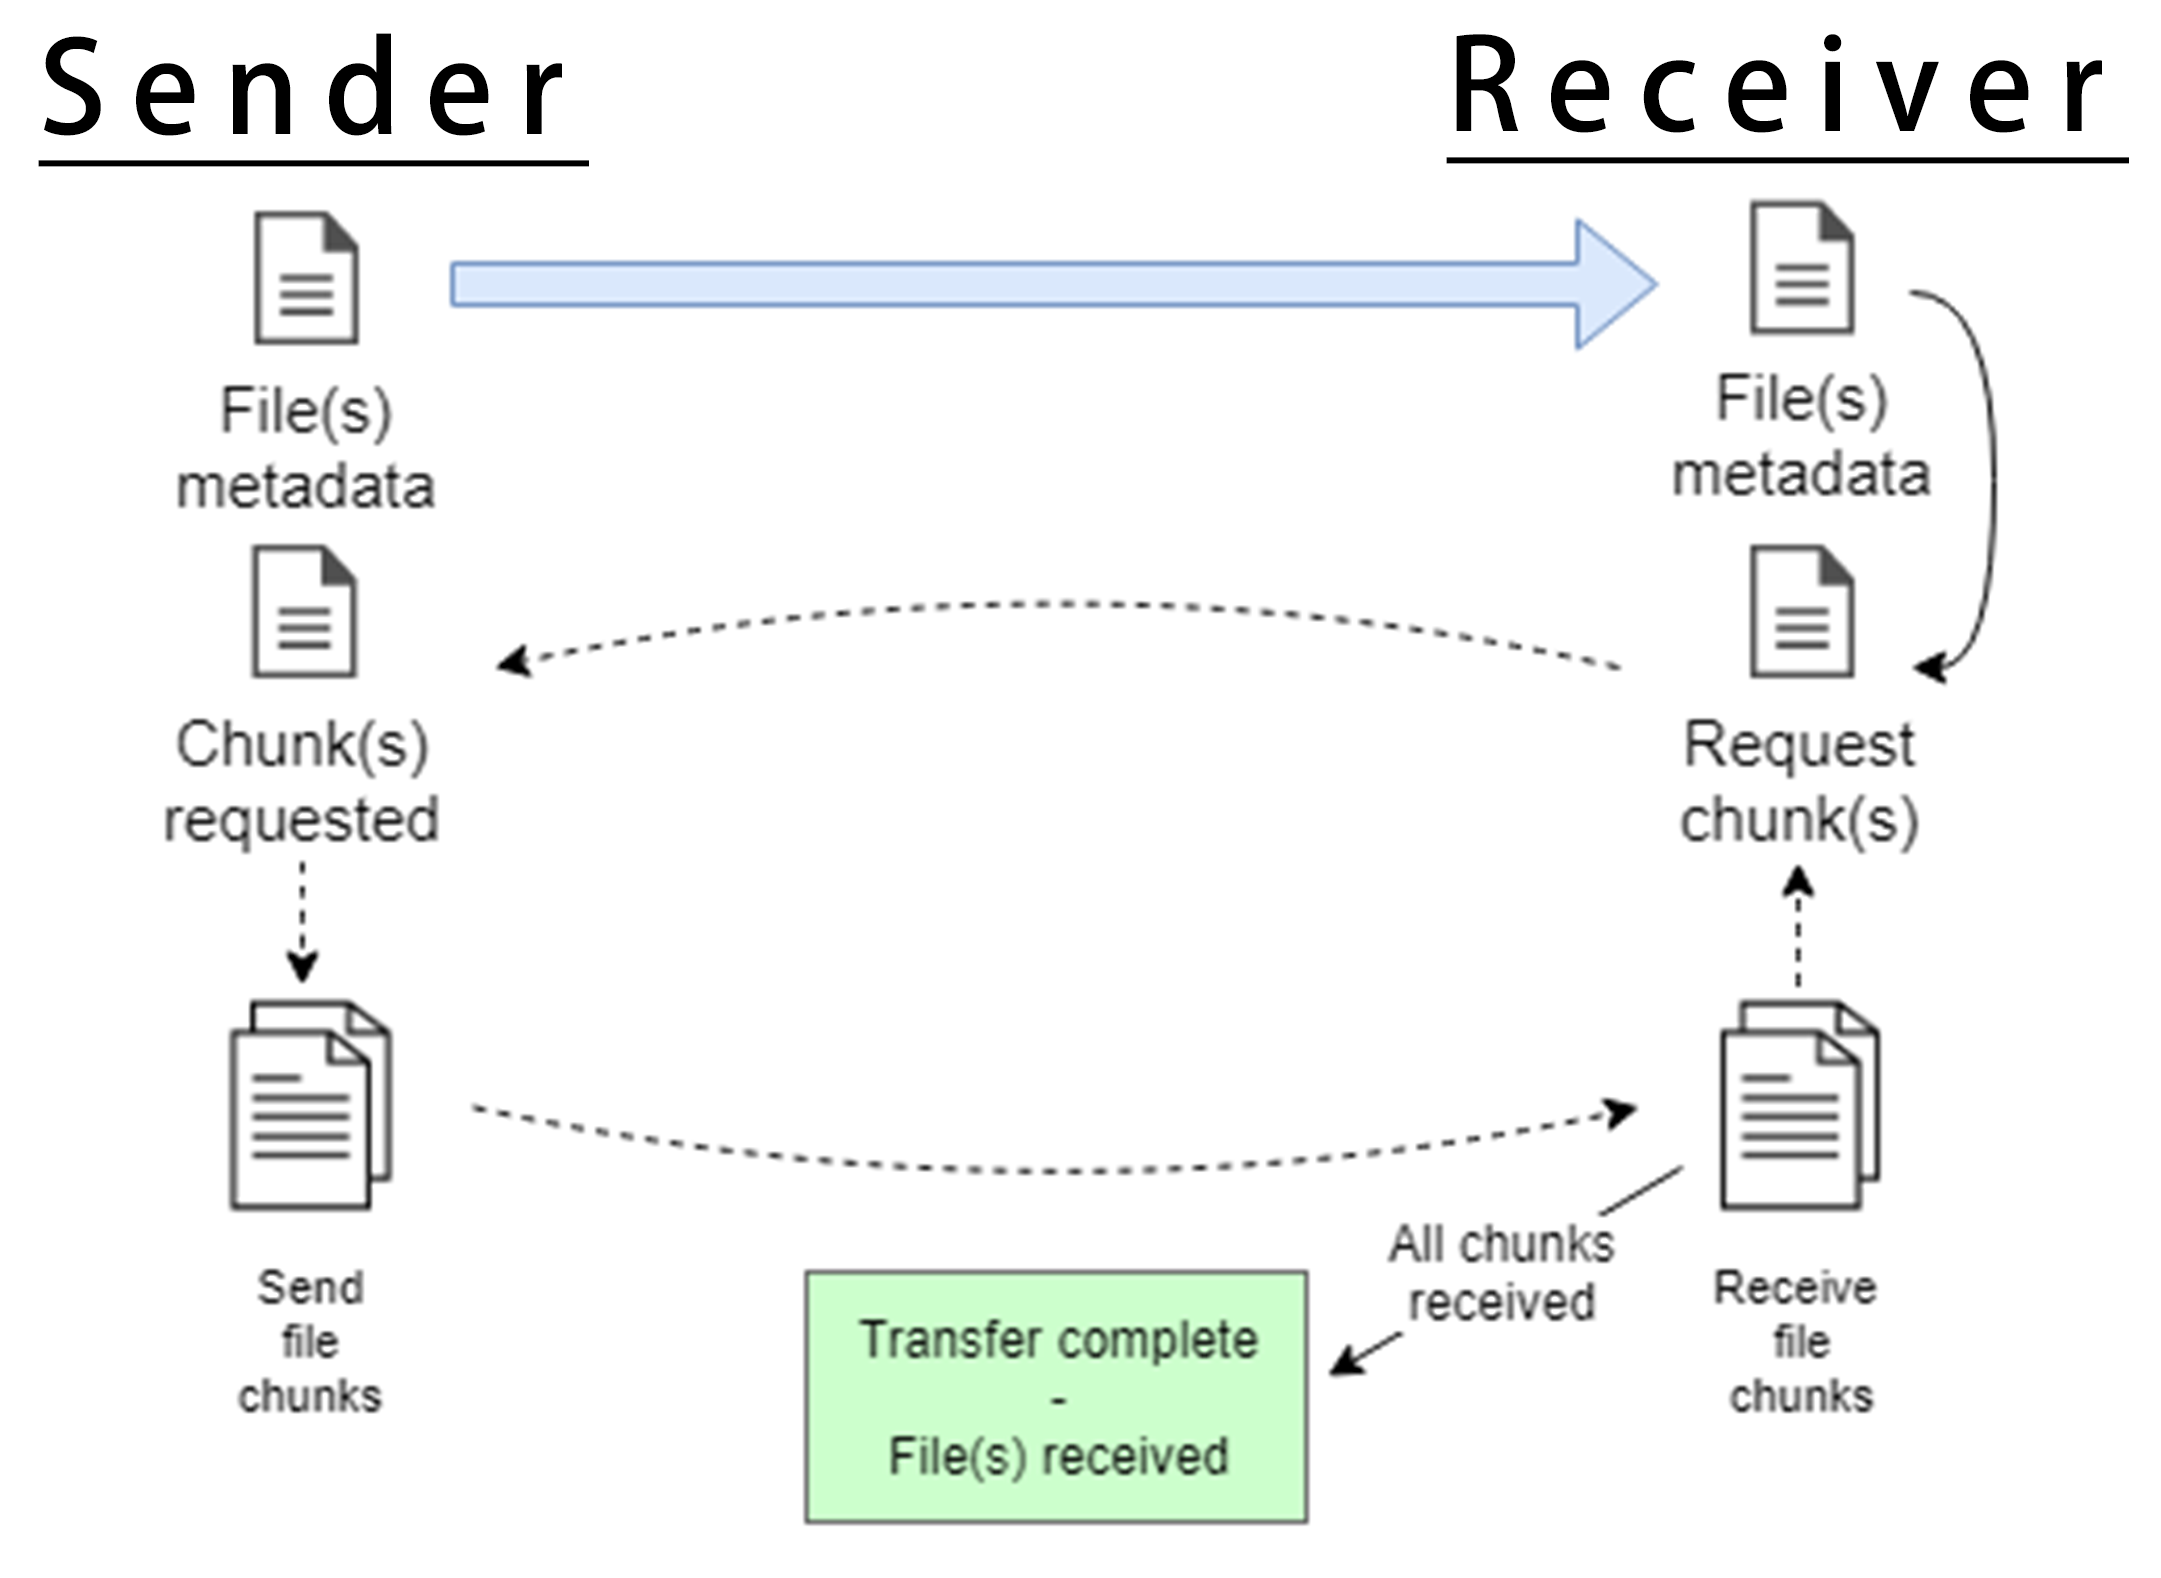
\includegraphics[width=100mm]{Figures/File_share_protocol}
		  \decoRule
		  \caption[File sharing process]{This illustrates the process of transferring file(s).}
		  \label{fig:file_off}
		\end{figure}

		The file is always transferred over a secure P2P channel and with end-to-end encryption. It is transferred using the protocol mentioned in the previous section, in order to manage the transfer.

		Implementing support for bigger files, which means additional chunking, should be relatively easy. As a result, transport of data larger than the current limitations, was not implemented. If this becomes necessary in the future, it can be added as an extra feature. For more on this subject, see \Cref{sec:bigfile}
		
		%File manager
		The chunking, as well as managing which files are to be sent and which files have been received, is done by the File Manager. The File Manager reads a file into memory, then separates the data into chunks. These chunks are then sent through the P2P channel. Once the recipient has received all the chunks, indicated by the metadata previously received, the transfer of that file is regarded as complete. This triggers the chunks to be combined into the original file, and then stored on the recipients computer. It also notifies the sender to start transfer of the next file, or that the transfer is complete.

	\subsection{Modes}
	%
		SendIt operates with two unique modes. One is the ACS mode, which acts as a helper in establishing the P2P connection. The other mode is the Serverless mode, which leaves it in the hands of the end user. What is important to note is that these modes can be selected as the user sees fit. It will also retain information used and gathered in one mode, and utilize it for future connections in the other mode. What it cannot do is transfer data from one endpoint in one mode, to another endpoint in a different mode. Both endpoints have to be in the same mode in order to be able to establish a connection. However, they can switch modes and still connect at a later time, as long as they both utilize the same mode. These modes will be further discussed in \Cref{Chapter5}.

\section{ACS server design}
	\label{sec:acs_serv_des}
	%ACS Server
	%
	The ACS server is in charge of forwarding information from one endpoint to another. It also has some other functionality, like authenticating identities, for the sake of forwarding information to the correct endpoint. The functionality of this server is kept minimal and, as such, should be easy to utilize. It is also easily extendable and deployable, which makes it easy for users to host their own, for their own needs, if they for any reason do not trust any available service.
%
	\subsection{Authentication}
	\label{sec:wsprot_auth}
	%Authentication
		%How? Setup? Usage?
		%
		\begin{figure}[th]
		  \centering
		  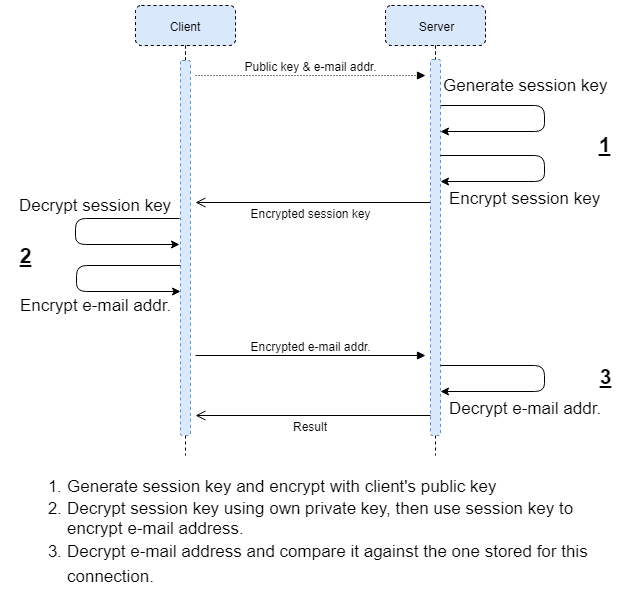
\includegraphics[width=\textwidth]{Figures/ACS_Prot/ACS_server_auth}
		  \decoRule
		  \caption[ACS server authentication scheme]{This figure illustrates how the ACS server authenticates clients. The initial transfer from client to server only happens if they are communicating for the first time.}
		  \label{fig:ACS_serv_auth}
		\end{figure}
		%
		The authentication scheme for the ACS server is extremely simple and just meant as an example for more sophisticated solutions. It works by having the ACS server create a symmetric key and encrypt it using the endpoint's public key. To prove to the server that the endpoint could decrypt the session key, it encrypts it's own identity (e-mail) using the symmetric key and sends it back. If the identity matches the one stored, then the endpoint is authenticated.

		If it is the first time an endpoint connects to the server, the endpoint shares their public key and identity with the server. The server then generates a symmetric key, encrypts it with the public key supplied, and shares it with the endpoint. The authentication scheme is illustrated in \Cref{fig:ACS_serv_auth}.
		
		The reason for incorporating this into the server is that forwarding data to the wrong endpoint could potentially reveal information not meant for that identity. As such, some basic form of authentication should be added to ensure that the information ends up at the right identity. This authentication does not replace or interfere with the regular authentication between endpoints in any way. It is simply a feature added to make sure the data arrives at the intended endpoint.
	%
	\subsection{Communication}
	%
	No code needs to be sent from the ACS server to the endpoint in order to communicate, since all the code is pre-programmed into the client software. As such, the server cannot manipulate nor control the clients behavior in any way, except that intended by the protocol. In this section, when WebRTC is specified, it can be substituted with any Offer/Answer based model or protocol.

	\subsection{ACS Protocol}
	\label{sec:wsprot}
	%
	\begin{figure}[th]
	  \centering
	  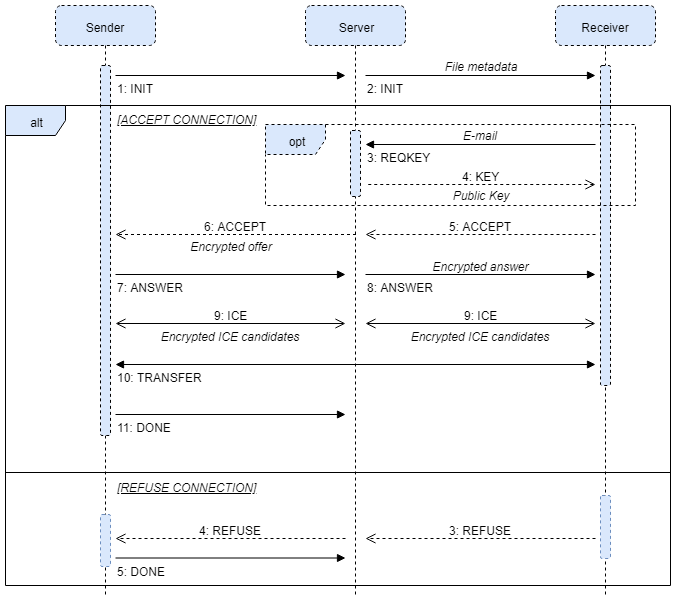
\includegraphics[width=\textwidth]{Figures/ACS_Prot/Communication}
	  \decoRule
	  \caption[ACS protocol: Communication]{This is the main functionality and flow when using ACS mode to transfer files. Do note that the area marked OPT is not implemented.}
	  \label{fig:prot_comm}
	\end{figure}

	%
	The protocol used to negotiate and broker a connection in the ACS mode is made specifically for use with Offer/Answer based protocols. It is kept as minimal as possible, with some of the functionality not yet implemented. This functionality is not necessary, but would improve the system. The basic format of every interaction is shown in \Cref{tab:basic}.

	For an overview of the general communication flow, once authenticated and properly connected, see \Cref{fig:prot_comm}. This is where the main functionality of the ACS server is shown. For information about the specific implementation of this protocol see \Cref{sec:prot_imp}.
	%
	\begin{table}
		\caption[ACS protocol: Basic format]{Basic protocol format}
		\label{tab:basic}
		\centering
		\begin{tabular}{l l l l}
	        \toprule
			\tabhead{Field Name} & \tabhead{Type} & \tabhead{Description} & \tabhead{Required} \\
			\midrule
			Function & String & Name of function & Yes\\
	        Origin & String & E-mail address & Yes\\
	        Destination & String & E-mail address & No\\
	        Data & JS Object & Relevant data & No\\
			\bottomrule\\
		\end{tabular}
	\end{table}
	%
	\paragraph{}
	%
	\begin{figure}[th]
	  \centering
	  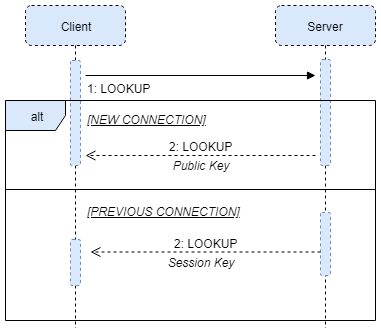
\includegraphics[width=80mm]{Figures/ACS_Prot/Connect}
	  \decoRule
	  \caption[ACS protocol: Lookup]{The lookup function exists so that the endpoint knows whether to start an authentication setup or an authentication process with the server.}
	  \label{fig:prot_lookup}
	\end{figure}

	\subsubsection*{Lookup}
	%SMALL PART IS IMP!
	The first interaction between the client and the server is the \emph{lookup} packet. The client connects to the server, and sends a \emph{lookup} packet containing the identity's e-mail address. If the server has previously communicated with the identity, it will create and send a session key (symmetric key) encrypted using the key associated with the identity. If it has not previously communicated with the identity, the servers public key is sent.

	The flow of this procedure is shown in \Cref{fig:prot_lookup}. This functionality is necessary so the endpoint knows if it should initiate an authentication setup (if there is no associated key in the server) or an authentication process (if there is an associated key in the server).

	%
	\begin{figure}[th]
	  \centering
	  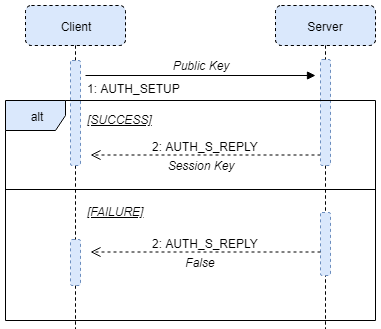
\includegraphics[width=80mm]{Figures/ACS_Prot/Auth_Setup}
	  \decoRule
	  \caption[ACS protocol: Authentication setup]{This shows how the authentication setup happens, and the data which is exchanged between the server and client in the two scenarios. The setup fails if the ACS server already has information stored for the given key or e-mail address.}
	  \label{fig:prot_setup}
	\end{figure}	

	\subsubsection*{Authentication setup}
	The authentication setup between a client and the ACS server is illustrated in \Cref{fig:prot_setup}. This happens the first time an identity communicates with an ACS server and allows the ACS server to be sure that it is always communicating with the same endpoint for any given identity. The endpoint sends it's public key, attached to an \emph{Authentication setup} packet, to the server. The server then checks if the e-mail is already registered. If it is, it notifies the endpoint by sending an \emph{Authentication setup reply} packet, indicating that the setup failed. If the setup is successful, the server sends a symmetric key attached to an \emph{Authentication setup reply} packet. This symmetric key is encrypted with the endpoint identity's public key, as part of the authentication. 

	%
	\begin{figure}[th]
	  \centering
	  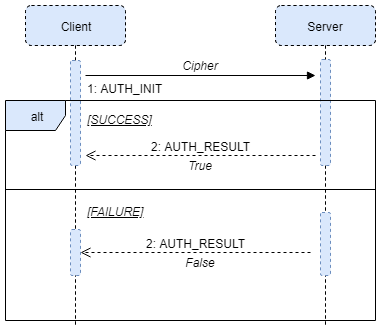
\includegraphics[width=80mm]{Figures/ACS_Prot/Auth_Init}
	  \decoRule
	  \caption[ACS protocol: Authentication]{This shows how the server authenticates the user. If the decrypted cipher matches the expected value, the authentication is successful.}
	  \label{fig:prot_auth}
	\end{figure}

	\subsubsection*{Authentication}
	The authentication is done as described in \Cref{sec:wsprot_auth}. The endpoint encrypts it's e-mail address using the symmetric key, and sends it to the server in the data field of an \emph{Authentication init} packet. The server then decrypts the cipher and compares the e-mail stored to the one received. If there is a match, the authentication is successful. If it does not match the connection is dropped. The result of the authentication is sent as part of the \emph{Authentication reply} packet. See \Cref{fig:prot_auth} for a diagram of this process. 
	
	\subsubsection*{Init}
	Once the endpoint has been authenticated by the server, it is available to receive offers and send offers. This is where the \emph{Init} functionality comes in. This is an offer to send files to an identity. It contains information about who the sender is, who the intended recipient is, and metadata about the file to be shared. See \Cref{fig:ACS_rec} for an example. If the server receives this type of request, it is forwarded to the indicated endpoint. The file metadata can be end-to-end encrypted without impacting the functionality.

	\subsubsection*{Accept}
	Once an endpoint receives an offer to receive files (in the form of an \emph{Init} packet), the user has the choice to accept or refuse the connection. If the user accepts, an \emph{Accept} packet containing a WebRTC Offer is sent back through the ACS server.

	\subsubsection*{Refuse}
	In the same way as explained for the \emph{Accept} functionality, the \emph{Refuse} functionality declines the offer to connect to the other endpoint. It terminates the connection setup between the two identities.

	\subsubsection*{Answer}
	If the Sender receives an \emph{Accept} packet, it means the other endpoint accepted the connection. As such, the Sender processes the WebRTC Offer received, and generates a WebRTC Answer. This is then shared back to the Recipient through the ACS server in the form of an \emph{Answer} packet.

	\subsubsection*{ICE}
	Since this solution utilizes ICE trickling (Described in \Cref{sec:webrtc_icetri}), it needs a protocol to continuously share ICE candidates between the two endpoints. This function exists to allow the sharing of such candidates. In other words, the ICE candidate is attached as the data portion of the \emph{ICE} packet.

	\subsubsection*{Done}
	This functionality indicates that the previous connection, for whatever reason, has ended. If one endpoint sends such a packet to the ACS server, the server should consider both endpoints available for new connections.

	\subsubsection*{Error}
	If for any reason an error occurs on either side, this functionality allows for sharing what went wrong with the other endpoint. As such, the reason for the error is added to the data portion of the packet. There is no requirement to share error messages with the connection partner, but it can be useful in order to discern between an intended pause/stop in the connection, or if something went wrong.

	\subsubsection*{Wait}
	This functionality is primarily aimed at allowing semi-asynchronous communication. It is used as a message to the endpoint from the ACS server, if they try to reach an identity currently connected to another endpoint. This indicates that the intended recipient is busy, but online. If one implements queuing, it can be used to tell the sender to wait until the endpoint is ready and then automatically connect.
%
	%Forwarding
	%
	\subsection{Forwarding}
	The ACS is a service that exclusively forwards information, regardless of whether it is encrypted or not. This is done by having the Sender, Recipient, and type of communication unencrypted. The server needs this information in order to handle the requests, and as such, these fields are left in cleartext. Using this information, the ACS picks the correct functionality and executes it. For most functionality, that means just forwarding the information to the correct endpoint. It does, however, need to authenticate the user and take care of that authentication setup, therefore it supports functionality beyond just forwarding information. While some of the data is unencrypted, it is important to note that the communications channel is encrypted, so an attacker cannot gain access to any of the data.
	
	%
	%Semi-asynchronous transfer
	%
	\subsection{Semi-asynchronous transfer}
	The ACS solution can allow for semi-asynchronous messaging. This means that one can issue the connection request at any time, but wait for it to be handled until the other endpoint comes online. It also allows for a queuing system that stores requests and handles them at the first available opportunity. This still requires the sender to be online, connected to the ACS, and available for transfer. As such, while the actual transfer is synchronous, the request and user interactions are not, thus 'semi-asynchronous'.

	This brought forward the need for the \emph{wait} and \emph{busy} functionality in the protocol, as well as a queue of jobs for each connection, temporarily kept in the ACS server. This type of transfer is not implemented in SendIt, but some of the frameworks and systems needed for such functionality is implemented and ready to be used.